\documentclass[a4paper,11pt]{scrartcl}

\usepackage[utf8]{inputenc}
%\usepackage[ngerman]{babel}
\usepackage[T1]{fontenc}
\usepackage{amsmath}
\usepackage[left=3cm, right=2cm, top= 2cm, bottom = 2.5cm, includeheadfoot]{geometry}
\usepackage[svgnames]{xcolor}
%\usepackage{gnuplottex}
\usepackage{pdfpages}
\usepackage{listings} 
\lstset{
	basicstyle=\scriptsize\color{Black},
	keywordstyle=\color{SteelBlue}\bfseries,
	language = C,
	numbers=right, numberstyle=\tiny, stepnumber=5, numbersep=0pt,
	showstringspaces=false}
\usepackage{url}
\usepackage{setspace}
%umgebungen sind \begin(singlespace/onehalfspace/doublespace)
%einfacher eineinhalbfacher und 2facher zeilenabstand
%es kann aber auch nur mit {\singlespace bla bla} {\doublespace blabla } und {\onehalfspacing} gearbeitet werden.

\usepackage{times}
\usepackage{graphicx}
\usepackage{color}
\usepackage{fancyhdr}
\pagestyle{fancy}
\lhead{{\small Simon Stadlinger, Jonas Kordt}}
\chead{Übungsserie 4}
\rhead{{\small Programmiertechnik II}}

\rfoot{}
\cfoot{\thepage}
\lfoot{}

%\pagestyle{headings}

%Befehle um Kopfund Fuszeile Anzupassen:
%\thepage - Seitennummer
%\leftmark - Aktueller Kapitelname "Kapitel X. Name des Kapitels"
%\rightmark - Aktueller Untertitelname "X.X Name des Kapitels
%\chaptername - Das Wort "Kapitel"
%\thechapter - Aktuelle Kapitelnummerierung
%\thesection - Aktuelle Unterkapitelnummerierung
%\slshape - Kursiv und Sanseriv
\title{Übung XX}

\begin{document}
\begin{center}
\LARGE{\textbf{Aufgabe 2}}
\end{center}
\paragraph{a)}$O(n^2)\subseteq O(n^3)$\\
g.z.z:
\begin{align*}
\forall a(n): a(n)\in O(n^2) \rightarrow a(n)\in O(n^3)
\end{align*}
sei 
\begin{align*}
&a(n)\in O(n^2)\\ &\rightarrow a(n)\leq c\cdot n^2 \\&\text{ab bestimmten n$_0$ und mit festem c ungleich 0}\\ &\text{da } c\cdot n^2 < c\cdot n^3 (n\in N, \text{Transitivität der kleinergleich-Relation})
\\ &\rightarrow a(n)<c\cdot n^3
\\ &\rightarrow a(n)\in O(n^3)
\end{align*}
q.e.d.
\paragraph{b)}$10\cdot n + 20 \in O(n)$ \\ g.z.z:
\begin{align*}
\exists c\in N, \exists n_0\in N: \forall n\geq n_0: 10\cdot n + 20 \leq c\cdot n
\end{align*}
Sei $c=11$
\begin{align*}
\exists n_0: \forall n\geq n_0: 10\cdot n +20 \leq 11\cdot n
\end{align*}
Dieses $n_0 = 20$. Es gilt
\begin{align*}
\Rightarrow\mbox{ }&\forall n\geq 20: 10\cdot n +20 \leq 11\cdot n\\
\Leftrightarrow\mbox{ }&\forall n\geq 20: 10\cdot n +20 \leq 10\cdot n + n\\
\Leftrightarrow\mbox{ }&\forall n\geq 20: n +2 \leq n + \frac{n}{10}\\
\Leftrightarrow\mbox{ }&\forall n\geq 20: 2 \leq \frac{n}{10}\\
\Leftrightarrow\mbox{ }&true
\end{align*}
q.e.d.
\paragraph{c)} $n^{\frac{2}{3}}\in O(n\cdot log(n))$\\ 
\begin{center}
Es gilt $n^{\frac{2}{3}} \in O(n)$ da $\forall n>n0:n^{\frac{2}{3}} < n^1$\\ Auch gilt $O(n)\subseteq O(n\cdot log(n))$ da die Laufzeit ab einem gewissen $n0\geq 1$ betrachtet wird  \\ Analog zu oben folgt daraus $n^{\frac{2}{3}}\in O(n\cdot log(n))$

\end{center}

Gut zu sehen ist dies auch in Figure 1.
\begin{figure}[h]
\begin{center}
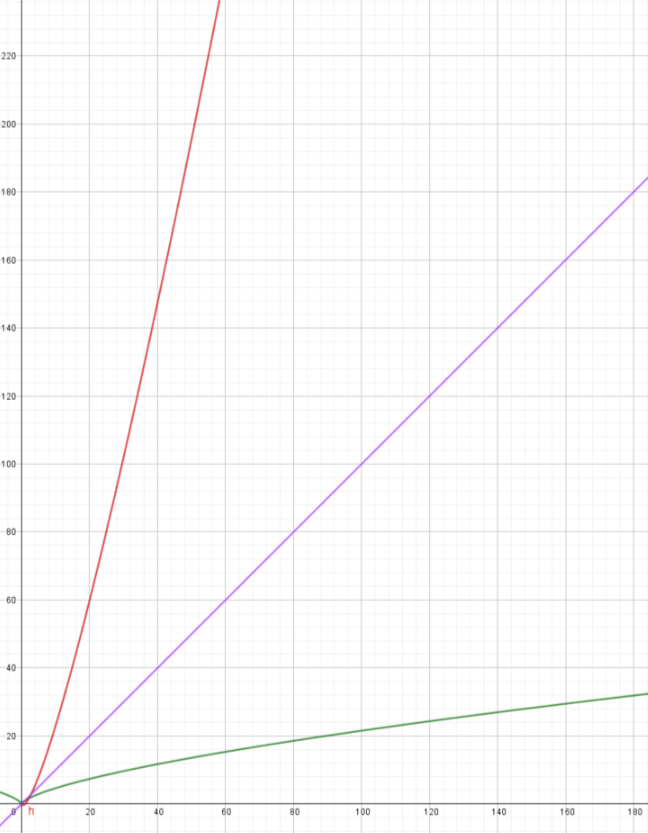
\includegraphics[scale=.7]{a2c_plot}
\caption{{\color{red} $h(n)=n\cdot log(n)$}, {\color{purple} $g(n)=n$}, {\color{DarkGreen} $h(n)=n^{\frac{2}{3}}$} }
\end{center}
\end{figure}
\end{document}
